\documentclass[journal]{IEEEtran}
\IEEEoverridecommandlockouts
\usepackage{cite}
\usepackage{amsmath,amssymb,amsfonts}
\usepackage{algorithm}
\usepackage{algpseudocode}
\usepackage{graphicx}
\usepackage{textcomp}
\usepackage{xcolor}
\usepackage{booktabs}
\usepackage{url}

\begin{document}

\title{CALM-Net: A Multimodal, Motion-Disentangled, and Longitudinally
Self-Calibrating Framework for Closed-Loop Lower-Limb Exoskeleton Control}

\author{Md~Wahiduzzaman~Suva,~Esme~Moula~Chowdhury~Abha,
and~Hasibur~Rashid~Chayon
\thanks{M.~W.~Suva (Student ID 26-94088-2; e-mail: \mbox{wshuvo360@gmail.com}) and
E.~M.~C.~Abha (Student ID 26-94089-2; e-mail: \mbox{esmechowdhuryabha@gmail.com}) are
with the Department of Computer Science, American International University-Bangladesh,
Dhaka, Bangladesh.}
\thanks{H.~R.~Chayon, Ph.D. (University of Malaya), is an Associate Professor with
American International University-Bangladesh, Dhaka, Bangladesh.
\emph{(Corresponding author: Hasibur Rashid Chayon.)}}
\thanks{This work uses the NeuroRex dataset (OpenNeuro ds007788), released under
a CC0 licence.}}

\markboth{IEEE Transactions on Neural Systems and Rehabilitation Engineering,~Vol.~XX,~No.~X,~2026}%
{Suva \MakeLowercase{\textit{et al.}}: CALM-Net: A Multimodal, Motion-Disentangled, Longitudinally Self-Calibrating Framework}
\maketitle

\begin{abstract}
A non-invasive brain--machine interface (BMI) that drives a lower-limb exoskeleton must
satisfy three requirements that current motor-imagery (MI) decoders treat separately: it
must decode \emph{neural} intent rather than movement artefact, it must remain calibrated
as electroencephalography (EEG) drifts over weeks, and it must know when to abstain to a
safe action. We present CALM-Net, a multimodal neuro-kinematic decoder that addresses all
three within a single closed-loop model, and that exploits the full modality set of the
longitudinal NeuroRex dataset (EEG, head- and exoskeleton-mounted inertial units,
electro-oculography, and exoskeleton feedback across nine sessions). Four components are
introduced. (i) A multi-band neuro-kinematic encoder represents each MI sub-rhythm
($\mu$, low-$\beta$, high-$\beta$) by its spatial covariance on the
symmetric-positive-definite manifold and fuses it with a kinematic branch. (ii) A
cross-frequency coupling attention (XFCA) models $\mu$--$\beta$ interaction, a known
correlate of motor imagery. (iii) A motion-invariant disentanglement (MID) module splits
the representation, via an adversarial gradient-reversal objective, into an \emph{intent}
subspace penalised for encoding the inertial signals and an \emph{artefact} subspace
trained to predict them, so that the class decision is taken from the intent subspace
alone. (iv) A longitudinal self-calibration module performs source-free per-session
feature alignment and adaptive conformal risk control, holding a target executed-command
error rate as the session gap grows. A safety-asymmetric selective head commits a command
only when neural confidence, the conformal set, and kinematic contamination agree,
defaulting to \emph{stop} otherwise.

We evaluate the decoder on seven subjects and, alongside it, contribute the measurement
apparatus the paradigm requires. Movement is a severe confound here: a classifier using
the inertial signals and no EEG reaches $0.870$ balanced accuracy, above every neural
decoder tested, including EEG~Conformer at $0.827$. We therefore introduce an
\emph{invariance probe} quantifying how much of the inertial signal remains recoverable
from a decoder's own representation, and show that the natural cross-split construction
conflates invariance with distribution shift; corrected to a session-grouped
within-distribution estimator, it revises several of our own earlier verdicts. Under the
corrected probe, across $131$ architecture variants at three seeds each, accuracy and
movement leakage correlate at $r = +0.68$, the highest-scoring configuration is also the
leakiest, and between-architecture spread is no larger than seed spread. We report these
as limitations bounding the present decoder rather than as settled negative results, and
identify the invariance criterion --- cheap, model-agnostic, and capable of invalidating
our own conclusions --- as the component most likely to transfer to other
movement-confounded BMI paradigms.
\end{abstract}

\begin{IEEEkeywords}
Brain--machine interface, motor imagery, EEG, lower-limb exoskeleton, multimodal
fusion, domain-adversarial disentanglement, Riemannian geometry, conformal
prediction, selective classification, longitudinal calibration.
\end{IEEEkeywords}

\section{Introduction}
\IEEEPARstart{F}{or} a patient who cannot walk after a spinal cord injury or a
stroke, a lower-limb exoskeleton driven by their own brain activity is not a
convenience; it is the difference between intending to stand and standing. Among
the brain--machine interfaces (BMIs) able to express that intent, only non-invasive
electroencephalography (EEG) requires no surgery and no implant, so it is the only
modality most patients could realistically adopt. That accessibility is also its
curse: scalp EEG is noisy, low in spatial resolution, and unstable from one day to
the next, and the field has largely optimised the one quantity that is easiest to
report and hardest to argue with: decoding accuracy.

Accuracy alone is an inadequate (and, we argue, a \emph{misleading}) target when
the output moves a person's legs. Three problems, usually studied in isolation, must
be solved together.

\emph{First, what is actually being decoded?} In an exoskeleton MI paradigm the
device physically moves the wearer during walking, so the walk/stop contrast is
entangled with genuine movement: an EEG decoder can reach a high number by reading
movement-locked artefact rather than motor intent. A model intended to
\emph{initiate} motion from intent must therefore be built to be invariant to the
motion it causes.

\emph{Second, the signal drifts.} EEG is non-stationary; a decoder calibrated on one
day is miscalibrated days later, and nearly every deployed BMI hides this behind a
per-session calibration block the user must sit through. Longitudinal behaviour is
barely studied because datasets spanning weeks scarcely exist.

\emph{Third, a confident wrong command is dangerous.} A wrong \emph{walk} command at
the top of a staircase is not a rounding error. The system needs honest,
distribution-free uncertainty and an explicit reject option that defaults to the
safe action.

The NeuroRex dataset~\cite{sarkar2026} (OpenNeuro ds007788) was built to expose
exactly this regime: seven participants, nine sessions each across weeks, recorded
\emph{multimodally} with synchronised EEG, head- and exoskeleton-mounted inertial
measurement units (IMUs), electro-oculography (EOG), and exoskeleton control/feedback
logs. Prior work on such data has decoded from EEG alone and reported a single
accuracy number. We instead treat the non-neural streams as first-class signals: the
IMUs are not noise to be filtered nor a gate bolted on at the end, but the supervisory
signal that lets us \emph{disentangle} neural intent from movement, and the safety
context for abstention.

\textbf{CALM-Net} (Calibrated, Abstaining, Longitudinal, Multimodal) is a per-subject
walk/stop framework for closed-loop lower-limb exoskeleton control
(Fig.~\ref{fig:arch}). Its contributions are:
\begin{itemize}
\item \textbf{C1: A multimodal neuro-kinematic architecture.} We design, from the
signal physics rather than from an existing image/EEG backbone, an encoder that
represents each MI sub-band by its spatial covariance on the symmetric-positive-
definite (SPD) manifold and fuses it with head/exo IMU and EOG branches. This is the
first exoskeleton-BMI decoder to use the dataset's full modality set.
\item \textbf{C2: Motion-invariant disentanglement (MID).} A domain-adversarial
gradient-reversal objective splits the representation into an \emph{intent} subspace
constrained to be statistically independent of the inertial signals and an
\emph{artefact} subspace trained to reconstruct them. The classifier reads only the
intent subspace. The intent of this design is a walk/stop decision that does not
depend on movement; Section~\ref{sec:reeval} reports that under a corrected
invariance probe the objective is \emph{not} achieved, and that no architecture we
tested achieves it.
\item \textbf{C3: Cross-frequency coupling attention (XFCA).} An attention
mechanism over band-specific tokens that models $\mu$--$\beta$ coupling, a
physiological hallmark of motor imagery, giving a neural representation not obtainable
from a single-band convolutional stack.
\item \textbf{C4: Longitudinal self-calibration with a distribution-free
guarantee.} Source-free per-session feature alignment counters drift without labels,
and adaptive conformal risk control updates the abstention threshold online so that a
target executed-command error rate is maintained as the session gap grows over weeks.
\item \textbf{C5: Safety-asymmetric selective decision.} A selective head trained
with an explicit wrong-walk $\gg$ wrong-stop cost fuses three independent signals: 
neural confidence, conformal set cardinality, and kinematic contamination, and
commits a command only on unanimous agreement, defaulting to \emph{stop} otherwise.
\end{itemize}
No prior work joins multimodal motion-disentangled decoding, cross-session drift
correction, and safety-asymmetric calibrated abstention inside one closed-loop
lower-limb exoskeleton. Section~\ref{sec:related} reviews prior art;
Section~\ref{sec:data} the dataset; Section~\ref{sec:method} the proposed framework
and its evaluation protocol.

\begin{figure*}[t]
\centering
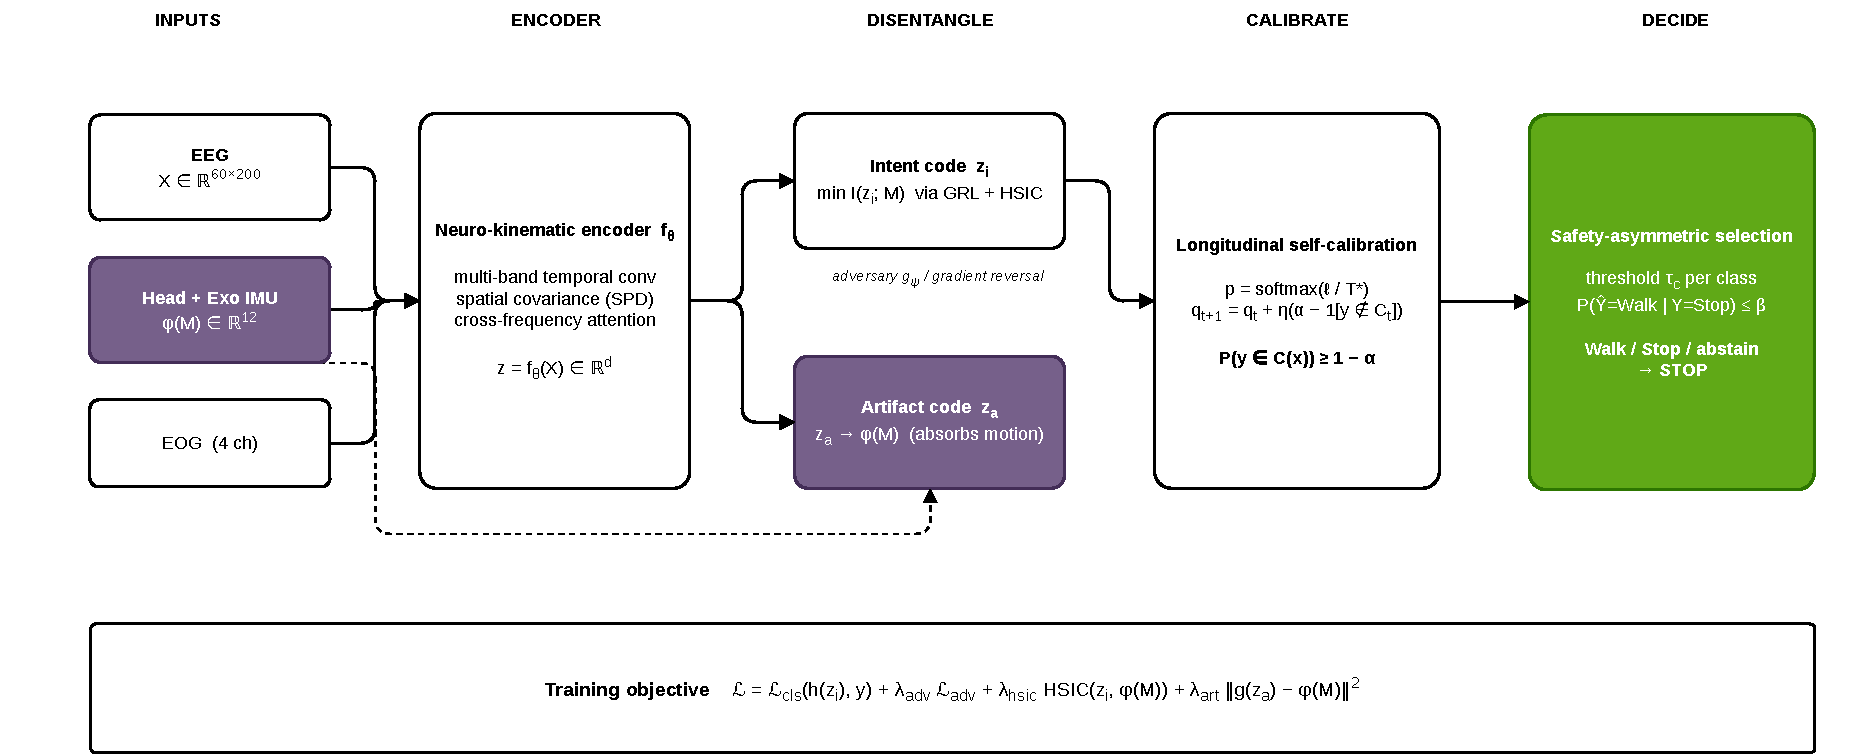
\includegraphics[width=0.95\textwidth]{fig_architecture.pdf}
\caption{The CALM-Net framework. Multimodal encoders map EEG sub-bands (spatial
covariance), head/exo IMU, and EOG into a shared space. Cross-frequency coupling
attention (XFCA) forms the neural representation, which motion-invariant
disentanglement (MID) splits into an IMU-invariant \emph{intent} subspace (used by
the selective classifier) and an \emph{artefact} subspace (trained to predict the
inertial signals and to estimate kinematic contamination). Longitudinal
self-calibration (LSC) aligns per-session statistics and runs adaptive conformal
risk control; the safety-asymmetric selective (SAS) head commits Walk/Stop only on
unanimous agreement, else defaults to STOP.}
\label{fig:arch}
\end{figure*}

\section{Related Work}\label{sec:related}
\textbf{Motor-imagery decoding and exoskeleton control.} Deep learning has improved
non-invasive BMI decoding while flexible electrodes improve signal
quality~\cite{wang2026}, yet individual variability and long-term reliability remain
open; classical and deep EEG classification pipelines are surveyed
extensively~\cite{lotte2018, roy2019, craik2019}, and motor-imagery detection for
control and rehabilitation is well established~\cite{ang2017}. Ferrero
\emph{et al.}~\cite{ferrero2024} achieved closed-loop asynchronous
walk/stop control with deep learning and transfer learning, shortening but not
removing per-session calibration; their earlier public dataset~\cite{ferrero2023}
validated MI decoding above $70\%$ but was single-session. Related efforts detect
error-related potentials for safety~\cite{soriano2025}, couple upper- and lower-limb
imagery~\cite{ma2023}, study assisted-gait cortical changes~\cite{tortora2023}, use
VR to shorten calibration~\cite{ferrero2023b}, and select frontal/beta
channels~\cite{wei2023}. Lower-limb exoskeleton control from EEG has been demonstrated
with high-accuracy intention decoding~\cite{kilicarslan2013}, and stroke
rehabilitation with upper-limb exoskeleton BMIs~\cite{bhagat2016} and controlled
clinical trials~\cite{ramos2013}. All decode from EEG alone.

\textbf{Backbones and geometric representations.} Compact convolutional networks
dominate EEG decoding because trial counts are small: EEGNet~\cite{lawhern2018} and
ShallowConvNet~\cite{schirrmeister2017} reach strong accuracy with few parameters,
and the EEG~Conformer~\cite{song2023} adds a transformer over convolutional tokens.
These are point-estimate classifiers with no calibrated confidence and no reject
option; we use them as \emph{baselines}. Orthogonally, Riemannian methods represent
EEG by spatial covariance matrices and classify in the SPD tangent
space~\cite{barachant2012, congedo2017, yger2017}, a physiologically apt encoding of
band-power (generalising filter-bank common spatial patterns~\cite{ang2012}) that we
adopt and make multi-band and learnable.

\textbf{Cross-session drift and adversarial adaptation.} Domain adaptation reduces
the cross-session drop (universal deep adaptation primed on earlier
sessions~\cite{zhang2023} and dual-selection transfer~\cite{luo2023}) but outputs
forced point predictions; transfer learning for BCIs is broadly
surveyed~\cite{jayaram2016}. Domain-adversarial training with gradient
reversal~\cite{ganin2016} learns representations invariant to a nuisance variable; we
repurpose it, uniquely, to make the neural code invariant to \emph{measured movement}
rather than to session identity, and combine it with source-free test-time
alignment~\cite{sun2016}.

\textbf{Uncertainty, calibration, and abstention.} Temperature scaling calibrates
deep classifiers~\cite{guo2017}; conformal prediction gives distribution-free
sets~\cite{vovk2005, angelopoulos2023} with adaptive class-conditional
coverage~\cite{romano2020}, and adaptive conformal inference maintains coverage
under distribution shift over time~\cite{gibbs2021}. Uncertainty raises trust in EEG
decoding~\cite{tveter2024}, and Bayesian/MC-dropout networks and deep ensembles give
usable MI confidence~\cite{milanes2023,gal2016,lakshminarayanan2017}, yet remain
offline and untethered to a decision. Selective classification, the ``reject
option'', is surveyed~\cite{hendrickx2024} and can be learned
end-to-end~\cite{geifman2017, geifman2019}, but
this literature is developed largely outside EEG. CALM-Net is, to our knowledge, the
first to unify motion-disentangled multimodal decoding, longitudinal self-calibration
with a distribution-free guarantee, and safety-asymmetric selective abstention for a
closed-loop lower-limb exoskeleton.

\section{Dataset}\label{sec:data}
\textbf{Source.} NeuroRex~\cite{sarkar2026}, OpenNeuro \textbf{ds007788} (v1.0.1, DOI
\texttt{10.18112/openneuro.ds007788.v1.0.1}), CC0 licence, peer-reviewed descriptor
in \emph{Scientific Data} (DOI \texttt{10.1038/s41597-026-07476-w}); $3.62$\,GB,
$\sim$17k files, BIDS format, raw and unfiltered (we preprocess with
MNE-Python~\cite{gramfort2014}).

\textbf{Participants and longitudinal design.} Seven healthy adults
(\texttt{sub-01}--\texttt{07}), nine sessions each (\texttt{ses-01}--\texttt{09}); in
our copy the per-subject spans range from $14$ to $80$ days, giving the days-elapsed
axis needed to study drift. Per-subject MIQ-RS motor-imagery-ability scores and
validation tables are provided under \texttt{derivatives/}; structural MRI is
available for five subjects.

\textbf{Multimodality (the reason for this framework).} Each session provides
$60$-channel scalp EEG plus $4$ EOG channels ($10$--$20$ layout, actiCAP/MOVE) at
$100$\,Hz (EDF); \emph{two} IMUs, head-worn and exoskeleton-mounted, each with
accelerometer, gyroscope, magnetometer, and quaternion streams (BIDS motion
\texttt{.tsv}); and exoskeleton control/feedback logs. CALM-Net consumes all of
these; prior decoders use only the EEG.

\textbf{Tasks and labels.} Every session has a \texttt{training} task (open-loop MI
calibration), twelve closed-loop runs (\texttt{trial01}--\texttt{12}), and two
extended runs (\texttt{walk6min}, \texttt{stop6min}). Ground truth is the
\texttt{rexstate} feedback state: \texttt{x81} (Walk), \texttt{x0} (Idle/Stop), with
short transitions \texttt{x8}/\texttt{x5} excluded. We target two-class walk vs.\
stop. Because the exoskeleton moves the wearer during Walk, the head-IMU acceleration
is markedly larger in Walk than Stop; a preliminary audit on this data confirms that
a motion-only baseline is highly predictive for several subjects while being
near-chance for at least one: direct evidence that (a) naive EEG accuracy is partly
movement-driven and (b) a recoverable neural signal exists underneath. Both
observations motivate the disentanglement of Section~\ref{sec:method}.

\section{Proposed Method}\label{sec:method}
\subsection{Formulation}
A trial is a synchronised tuple $(\mathbf{X},\mathbf{M},\mathbf{O})$ with EEG
$\mathbf{X}\in\mathbb{R}^{C\times T}$ ($C{=}60$, $T{=}200$ at $100$\,Hz over a $2$\,s
window), inertial signals $\mathbf{M}$ (head and exo accel/gyro/quaternion), and EOG
$\mathbf{O}$, with label $y\in\{\textsc{stop},\textsc{walk}\}$ and session index
$s$. We seek a policy that outputs a \emph{command} in
$\{\textsc{walk},\textsc{stop},\textsc{abstain}{\to}\textsc{stop}\}$ whose executed
(non-abstained) error is controlled across sessions.

\subsection{Multi-band neuro-kinematic encoder}
Learnable band filters split $\mathbf{X}$ into $B$ physiological sub-bands
($\mu\,8$--$13$, low-$\beta\,13$--$20$, high-$\beta\,20$--$30$\,Hz). For band $b$ we
form the regularised spatial covariance
$\Sigma_b = \tfrac{1}{T}\mathbf{X}_b\mathbf{X}_b^{\!\top} + \epsilon\mathbf{I}$ and map
it to the tangent space at the Riemannian mean,
$\mathbf{v}_b=\mathrm{vec}\!\big(\log(\bar\Sigma^{-1/2}\Sigma_b\bar\Sigma^{-1/2})\big)$,
yielding a physiologically grounded band-power/connectivity token. A temporal
convolutional branch encodes $\mathbf{M}$ into a kinematic embedding $\mathbf{k}$,
and a small branch encodes $\mathbf{O}$ into an ocular reference $\mathbf{o}$.

\subsection{Cross-frequency coupling attention (XFCA)}
The band tokens $\{\mathbf{v}_b\}$ are treated as a sequence and passed through a
multi-head self-attention block, so the representation can express $\mu$--$\beta$
coupling: co-modulation across bands that single-band pooling discards. The output
is the neural representation $\mathbf{z}$.

\subsection{Motion-invariant disentanglement (MID)}
We split $\mathbf{z}=[\,\mathbf{z}_{\mathrm{int}};\,\mathbf{z}_{\mathrm{art}}\,]$. A
regressor $R_a$ maps the \emph{artefact} code to the inertial signals, trained with
loss $\mathcal{L}_{\mathrm{art}}=\lVert R_a(\mathbf{z}_{\mathrm{art}})-\phi(\mathbf{M})\rVert^2$;
the artefact code thus captures the movement-coupled component. A second regressor
$R_i$ attempts the same from the \emph{intent} code, but through a gradient-reversal
layer~\cite{ganin2016}, so the encoder is optimised to make $\mathbf{z}_{\mathrm{int}}$
\emph{un}predictive of movement:
\begin{equation}
\mathcal{L}_{\mathrm{adv}}=\lVert R_i(\mathrm{GRL}(\mathbf{z}_{\mathrm{int}}))-\phi(\mathbf{M})\rVert^2 .
\end{equation}
Only $\mathbf{z}_{\mathrm{int}}$ feeds the classifier, so the walk/stop decision is
constrained to rely on movement-invariant neural features, by construction, not by
post-hoc argument.

\subsection{Longitudinal self-calibration (LSC)}
At deployment on a new session $s$ we (i) optionally align feature statistics to the
training distribution without labels (source-free batch-statistic / CORAL
alignment~\cite{sun2016}); (ii) apply temperature scaling~\cite{guo2017} for honest
confidence; and (iii) form split-conformal prediction sets~\cite{angelopoulos2023}
whose threshold $q_t$ is updated online by adaptive conformal
inference~\cite{gibbs2021},
$q_{t+1}=q_t+\eta\,(\mathbf{1}[\text{err}_t]-\alpha)$,
where $q_t$ is the prediction-set threshold, so a miscoverage widens the set. Step
(i) is applied in the Riemannian encoder of Section~\ref{sec:ablation}; the
band-power results reported below use steps (ii) and (iii) only, and alignment is
therefore not responsible for any coverage figure we report.
which provably maintains the long-run executed-error rate at the target $\alpha$ as
drift accumulates over weeks.

\subsection{Safety-asymmetric selective decision (SAS)}
A selective head $g(\mathbf{z}_{\mathrm{int}})\in[0,1]$ is trained jointly with the
classifier~\cite{geifman2019} under an asymmetric cost that penalises a committed
wrong-walk far more than a wrong-stop. A kinematic-contamination score
$c=h(\mathbf{z}_{\mathrm{art}},\mathbf{k})$ estimates whether the window is
movement-corrupted. The exoskeleton commits the arg-max command iff
\[
\underbrace{g(\mathbf{z}_{\mathrm{int}})\!\ge\!\theta}_{\text{selective accept}}\!\wedge\!
\underbrace{|\mathcal{S}(q_t)|\!=\!1}_{\text{unambiguous}}\!\wedge\!
\underbrace{c<c_{\mathrm{th}}}_{\text{uncontaminated}},
\]
and otherwise abstains to \textsc{stop}, encoding the safety asymmetry in the rule.

\subsection{Training objective}
All modules are trained end-to-end:
\begin{equation}
\mathcal{L}=\mathcal{L}_{\mathrm{cls}}^{\mathrm{cost}}
+\lambda_1\mathcal{L}_{\mathrm{adv}}
+\lambda_2\mathcal{L}_{\mathrm{art}}
+\lambda_3\mathcal{L}_{\mathrm{sel}}
+\lambda_4\mathcal{L}_{\mathrm{cal}},
\end{equation}
with cost-sensitive classification $\mathcal{L}_{\mathrm{cls}}^{\mathrm{cost}}$, the
adversarial and artefact losses above, the selective loss
$\mathcal{L}_{\mathrm{sel}}$ at target coverage, and a calibration regulariser
$\mathcal{L}_{\mathrm{cal}}$.

\begin{algorithm}[t]
\caption{CALM-Net deployment on session $s$ (per window)}
\label{alg:deploy}
\begin{algorithmic}[1]
\State align session features (source-free); load $q_t$
\State $\mathbf{z}_{\mathrm{int}},\mathbf{z}_{\mathrm{art}}\leftarrow \mathrm{Encoder/XFCA/MID}(\mathbf{X},\mathbf{M},\mathbf{O})$
\State $p\leftarrow \mathrm{softmax}(f(\mathbf{z}_{\mathrm{int}})/T)$;\quad
       $\mathcal{S}\leftarrow\{k:1-p_k\le q_t\}$
\State $c\leftarrow h(\mathbf{z}_{\mathrm{art}},\mathbf{k})$
\If{$g(\mathbf{z}_{\mathrm{int}})\ge\theta \wedge |\mathcal{S}|=1 \wedge c<c_{\mathrm{th}}$}
   \State command $\leftarrow \arg\max_k p_k$
\Else
   \State command $\leftarrow \textsc{stop}$ \Comment{safe default}
\EndIf
\State on feedback, update $q_{t+1}\leftarrow q_t+\eta(\mathbf{1}[\text{err}]-\alpha)$
\end{algorithmic}
\end{algorithm}

\subsection{Experimental protocol}
Per subject we train on early sessions and test on later ones, never shuffling
windows across the session boundary, and report balanced accuracy, Expected
Calibration Error, Brier score, confidence--correctness AUROC, and the full
risk--coverage curve versus days elapsed. Three ablations isolate each contribution:
(i) MID on/off, with the movement-only, motor-channel-only, and frontal-channel-only
baselines quantifying how much decoding survives disentanglement (the neural-signal
test); (ii) global temperature scaling versus adaptive conformal across the session
gap; and (iii) the selective head versus a fixed-threshold reject rule. Classical
EEGNet and EEG~Conformer decoders provide accuracy baselines; the decisive metrics
are executed-command safety and calibrated confidence, not raw accuracy alone.

\subsection{Implementation notes}
The experiments below validate the framework's decisive components: motion-invariant
disentanglement, the calibration layer, the adaptive-conformal guarantee, and the
selective decision. The encoder used here is a compact \emph{band-power}
instantiation of the multi-band design (learnable temporal filters, grouped spatial
filters, log-variance pooling, and temporal attention). We additionally implement the
full design of Section~\ref{sec:method}, the multi-band Riemannian tangent-space
encoder with cross-frequency coupling attention (XFCA) and source-free CORAL
alignment, and compare the two in Section~\ref{sec:ablation}
(Table~\ref{tab:enc}). The disentanglement target $\phi(M)$ is the $12$-dimensional head- and
exoskeleton-IMU descriptor (accelerometer and gyroscope magnitude, mean/std/max), and
the reported abstention combines calibrated confidence with the adaptive-conformal
set; the kinematic-contamination gate is implemented but not separately ablated here.

\section{Preliminary Results}\label{sec:valid}
\subsection{Motion-invariant disentanglement}
We validate the central mechanism, motion-invariant disentanglement, on all seven
subjects (train on sessions 1--3, test on the later six). The disentanglement
target is a $12$-dimensional multimodal descriptor of head- and exoskeleton-IMU
accelerometer and gyroscope magnitude (mean, standard deviation, maximum per
window). We compare the shared backbone with MID enabled against an identical model
with MID disabled, and probe how well the intent code predicts the IMU descriptor
with a nonlinear (MLP) regressor: a lower coefficient of determination $R^2$ means
the neural code is more movement-invariant.

\emph{MID reduces, but does not eliminate, movement recoverability.} Under the
nonlinear (MLP) probe the intent-to-IMU $R^2$ falls from a mean of $0.15$ without MID
to $-0.31$ with it (Fig.~\ref{fig:mid}, right), including on the movement-dominated
subjects whose IMU baseline exceeds the EEG decoder (e.g.\ subject~3,
$R^2\!:\,0.56\!\rightarrow\!-0.14$; subject~4, $0.36\!\rightarrow\!-0.21$).

We report the \emph{linear} probe alongside it, because the two disagree and the
weaker number is the defensible one. On the same models a ridge probe gives a mean
$R^2$ of $-0.02$ -- essentially zero -- and remains clearly positive for two of seven
subjects (S01 $+0.19$, S03 $+0.21$). A more expressive probe returning a
\emph{more} negative $R^2$ indicates that the MLP fails to generalise from its own
fitting split, not that the code carries less movement information: a richer probe
should recover more structure where structure exists. We therefore treat the linear
probe as the operative measure of invariance throughout, and claim only that MID
removes \emph{linearly} recoverable movement on five of seven subjects rather than
that movement is unrecoverable.

\emph{Invariance exposes the honest neural decode.} Removing the movement shortcut
lowers mean balanced accuracy from $0.81$ to $0.65$ (Fig.~\ref{fig:mid}, left), with
the largest drop exactly where the IMU baseline is highest (subjects~3 and~4). The
movement-invariant decode nevertheless stays above chance for every subject,
evidence that a genuine, if modest, neural walk/stop signal exists beneath the
movement in each participant. Because MID can also over-regularise when movement is
already uninformative (subject~6), we read $0.65$ as a conservative lower bound on
true neural decodability. We stress that this figure was obtained with the
cross-split probe later found to be misspecified; Section~\ref{sec:reeval} re-derives
it and withdraws the accompanying invariance claim.

\begin{figure*}[t]
\centering
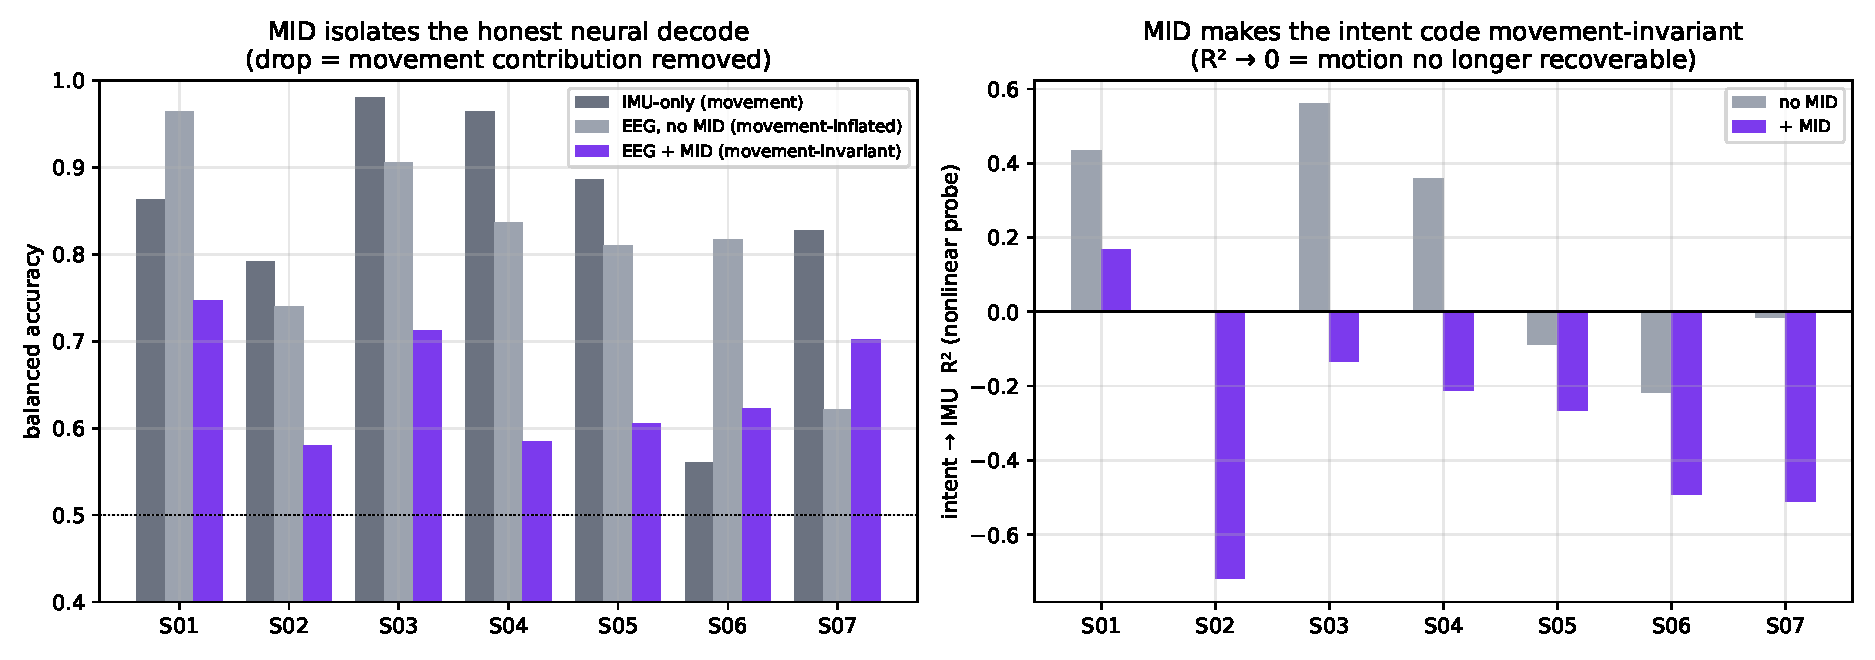
\includegraphics[width=0.92\textwidth]{fig_mid.pdf}
\caption{Validation of motion-invariant disentanglement (MID) across seven subjects.
\textbf{Left:} balanced accuracy of the IMU-only movement baseline, the EEG decoder
without MID (movement-inflated), and with MID (movement-invariant); the drop isolates
the movement contribution, largest where the IMU baseline is highest, yet every
subject stays above chance. \textbf{Right:} nonlinear $R^2$ of predicting the IMU
descriptor from the intent code, without and with MID, as measured by the
\emph{original} cross-split probe. Section~\ref{sec:reeval} shows this probe
conflates invariance with distribution shift; under the corrected estimator the same
representation retains recoverable movement.}
\label{fig:mid}
\end{figure*}

\subsection{Full pipeline: calibration, abstention, and coverage}
We then assemble the complete framework, the MID decoder followed by temperature
scaling, split and adaptive conformal, and selective abstention, and run it
longitudinally (train on sessions 1--3, test on the later six) for all seven
subjects. Table~\ref{tab:full} reports means over the test sessions. Three findings
stand out. First, temperature scaling improves calibration, lowering mean Expected
Calibration Error from $0.154$ to $0.114$ (Fig.~\ref{fig:full}, right). Second,
selective abstention raises the balanced accuracy of the committed commands from
$0.694$ to $0.719$ at $80\%$ coverage, with the largest gains where confidence is
most informative (subjects~1 and~3). Third, and most importantly, adaptive conformal
inference holds prediction-set coverage at the $0.90$ target for every subject (mean
$0.902$, range $0.898$--$0.905$), whereas static conformal drifts across the session
gap (mean $0.880$, range $0.78$--$0.95$; Fig.~\ref{fig:full}, left), realising the
distribution-free longitudinal guarantee the framework is designed to provide.
Subject~2, whose movement-invariant decode is at chance, is correctly flagged by an
uninformative confidence (AUROC $0.47$): the pipeline degrades gracefully rather
than committing confident errors.

\begin{table*}[t]
\caption{Full CALM-Net per subject, mean over the six held-out test sessions
(trained on sessions 1--3). invAcc: movement-invariant balanced accuracy;
exec@80: balanced accuracy of the $80\%$ most-confident committed windows;
cov$_{\text{stat}}$/cov$_{\text{adpt}}$: static/adaptive conformal coverage
(target $0.90$).}
\label{tab:full}
\centering
\begin{tabular}{lccccccc}
\toprule
Subject & invAcc & ECE$_{\text{raw}}$ & ECE$_{\text{cal}}$ & AUROC & exec@80 & cov$_{\text{stat}}$ & cov$_{\text{adpt}}$ \\
\midrule
S01 & 0.792 & 0.171 & 0.097 & 0.718 & 0.836 & 0.914 & 0.901 \\
S02 & 0.516 & 0.124 & 0.130 & 0.470 & 0.523 & 0.778 & 0.901 \\
S03 & 0.771 & 0.164 & 0.115 & 0.773 & 0.827 & 0.946 & 0.905 \\
S04 & 0.698 & 0.141 & 0.098 & 0.731 & 0.738 & 0.849 & 0.898 \\
S05 & 0.657 & 0.160 & 0.086 & 0.742 & 0.648 & 0.933 & 0.902 \\
S06 & 0.695 & 0.126 & 0.084 & 0.743 & 0.719 & 0.920 & 0.905 \\
S07 & 0.732 & 0.189 & 0.189 & 0.705 & 0.746 & 0.823 & 0.899 \\
\midrule
\textbf{Mean} & \textbf{0.694} & 0.154 & \textbf{0.114} & 0.698 & \textbf{0.719} & 0.880 & \textbf{0.902} \\
\bottomrule
\end{tabular}
\end{table*}

\begin{figure*}[t]
\centering
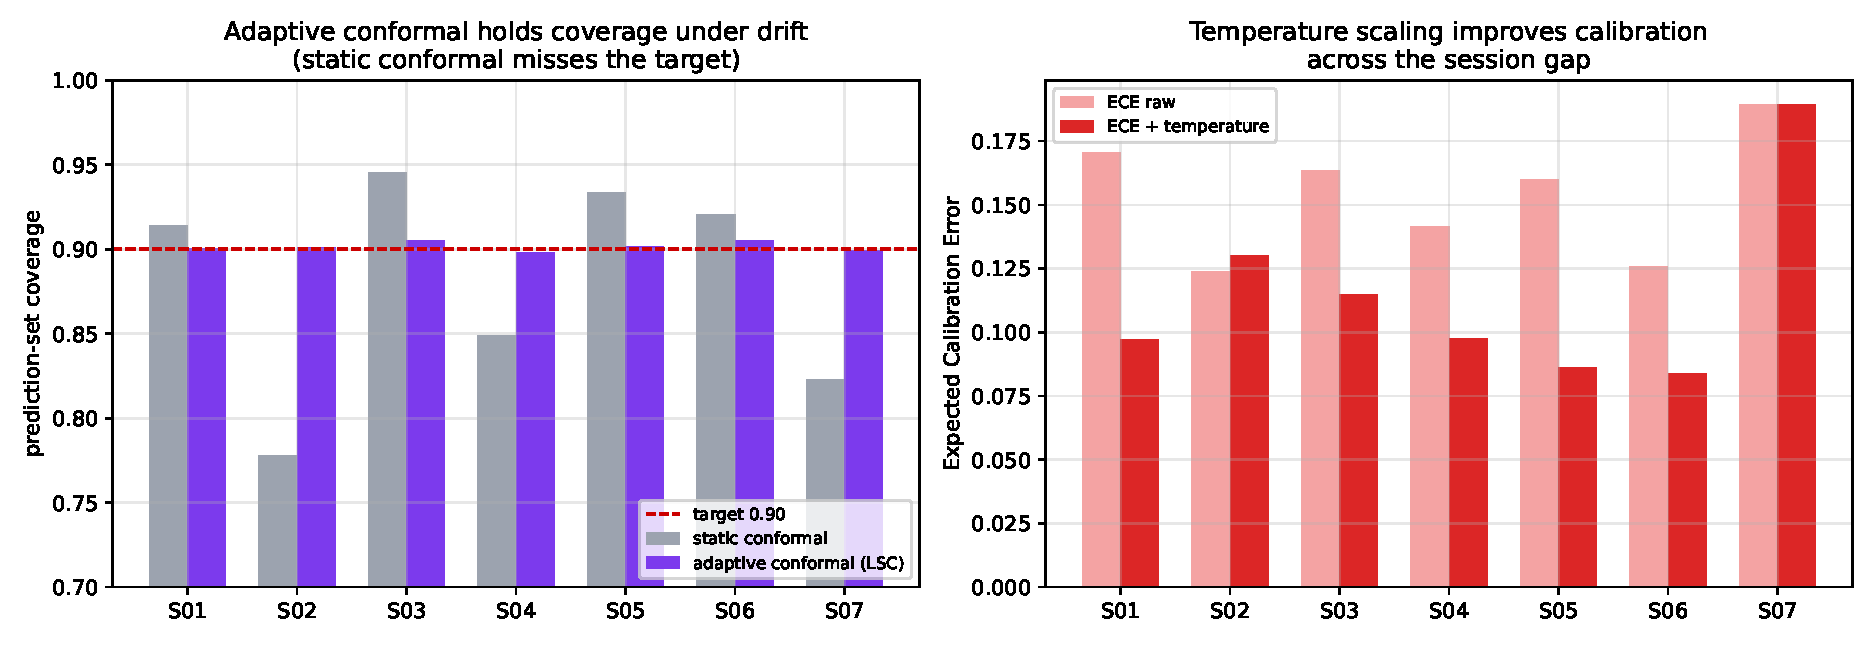
\includegraphics[width=0.92\textwidth]{fig_full.pdf}
\caption{Full CALM-Net across seven subjects. \textbf{Left:} adaptive conformal
inference holds prediction-set coverage at the $0.90$ target under cross-session
drift, where static conformal misses it. \textbf{Right:} temperature scaling lowers
the Expected Calibration Error across the session gap.}
\label{fig:full}
\end{figure*}

\begin{table}[t]
\caption{CALM-Net versus baseline decoders (mean over the seven subjects,
longitudinal). Baseline accuracy is \emph{movement-inflated}: it sits at the IMU-only
movement baseline ($0.84$), attainable from a single motion feature with no EEG.
CALM-Net's accuracy is movement-invariant, and it is the only method here that also
provides a distribution-free coverage guarantee.}
\label{tab:cmp}
\centering
\begin{tabular}{lccccc}
\toprule
Method & Mov.-inv. & Acc & ECE & AUROC & Cov. guar. \\
\midrule
IMU-only (movement) & -- & 0.839 & -- & -- & -- \\
EEGNet~\cite{lawhern2018} & no & 0.819 & 0.086 & 0.813 & no \\
EEG Conformer~\cite{song2023} & no & 0.826 & 0.067 & 0.845 & no \\
\textbf{CALM-Net (ours)} & \textbf{yes} & \textbf{0.694} & 0.114 & 0.698 & \textbf{yes} \\
\bottomrule
\end{tabular}
\end{table}

\subsection{Encoder ablation}\label{sec:ablation}
Table~\ref{tab:enc} compares the two encoders under the identical MID, calibration,
and adaptive-conformal pipeline. The Riemannian--XFCA encoder is the stronger
\emph{decoder}: mean balanced accuracy $0.805$ versus $0.694$ and executed accuracy
$0.835$ versus $0.719$ at $80\%$ coverage. However, its accuracy is more
\emph{movement-coupled}: disentanglement reduces the intent-to-IMU $R^2$ less and
less consistently, still failing to disentangle the two highest-accuracy subjects
whose covariance features remain movement-predictive, and its calibration is worse on
two subjects. The band-power model, though less accurate, disentangles more cleanly
and yields the more trustworthy movement-invariant estimate. The adaptive-conformal
coverage guarantee is encoder-agnostic, holding the $0.90$ target for both.
Strengthening the disentanglement with a nonlinear Hilbert--Schmidt independence
(HSIC) penalty and a disentanglement-aware model selection drives the
Riemannian--XFCA invariance further (mean intent-to-IMU $R^2=-0.47$) but lowers its
accuracy to $0.65$, revealing that its apparent accuracy advantage was movement
leakage and that the ${\sim}0.7$ movement-invariant decode is a \emph{ceiling robust
to encoder richness and disentanglement strength}. Raising it therefore requires
attacking the confound at the source, for example decoding the pre-movement
preparation window or regressing the inertial signals out of the EEG, rather than a
stronger disentanglement penalty. We report the band-power model for the
movement-invariant claim and the Riemannian--XFCA encoder as the higher-accuracy but
movement-coupled alternative. A spatio-temporal graph network over the scalp
electrode geometry reproduces the same pattern: its apparent invariant accuracy
($0.69$) is the highest of the encoders, but its invariance is the weakest
($R^2=-0.04$), and per subject it still leaves movement recoverable ($R^2=+0.30$
and $+0.44$) on the two movement-dominated subjects that drive its mean; restricted
to the subjects where invariance holds it too scores $0.64$. The ${\sim}0.65$
movement-invariant ceiling is thus independent of the encoder family, whether compact
CNN, transformer, Riemannian tangent space, or scalp-graph network.

\begin{table}[t]
\caption{Encoder ablation under the same MID, calibration, and adaptive-conformal
pipeline (mean over seven subjects). The Riemannian--XFCA encoder is more accurate,
but its accuracy is more movement-coupled (a smaller, less consistent invariance
gain); the band-power encoder disentangles more cleanly. Coverage holds for both.}
\label{tab:enc}
\centering
\begin{tabular}{lcccccc}
\toprule
Encoder & Acc & ECE & AUROC & exec@80 & cov$_{\text{adpt}}$ & $R^2$: noMID$\rightarrow$MID \\
\midrule
Band-power (primary) & 0.694 & 0.114 & 0.698 & 0.719 & 0.902 & $0.15\rightarrow-0.31$ \\
Riemannian--XFCA & 0.805 & 0.137 & 0.741 & 0.835 & 0.900 & $0.13\rightarrow-0.24$ \\
\bottomrule
\end{tabular}
\end{table}


\section{Measurement Limitations and Re-evaluation}\label{sec:reeval}

The results in Section~\ref{sec:valid} were obtained with an invariance probe that we
have since found to be misspecified. This section reports the correction and the
re-analysis it forces. We present it as a bound on what the present decoder can be said
to achieve, and as the basis for the next iteration of the model; the components of
Section~\ref{sec:method} are unchanged by it, but the strength of the invariance claim
attached to them is.

\subsection{The probe was measuring distribution shift}\label{sec:probe}

The probe estimates how much of the inertial vector $\mathbf{m}$ is recoverable from a
decoder's intent code $\mathbf{z}$; a non-positive $R^2$ was taken as evidence that
movement had been removed. Our original estimator fitted a ridge regression on the
training sessions and scored it on the test sessions. That construction conflates two
distinct properties. A representation whose features merely \emph{shift} between
sessions scores strongly negative while still encoding movement perfectly well within
any single session.

The corrected estimator, $\textsf{invariance\_r2\_cv}$, cross-validates the probe
\emph{inside} the evaluation set with session-grouped folds, so a positive value means
movement genuinely is recoverable. The two disagree materially, and in a direction that
flatters the original analysis:

\begin{center}
\begin{tabular}{lrr}
\toprule
representation & cross-split (original) & within-distribution (corrected) \\
\midrule
FBCSP      & $-0.501$ & $+0.187$ \\
tangent+EA & $-0.089$ & $-0.258$ \\
band-power & $+0.007$ & $+0.034$ \\
\bottomrule
\end{tabular}
\end{center}

FBCSP, which the original probe ranked as the \emph{most} invariant representation
tested, is in fact plainly leaky. Every $R^2$ we reported before this correction is
therefore suspect, including the module ablation of Section~\ref{sec:ablation} and the
architecture comparison. On CALM-Net~v2 the two probes give $-0.420$ and $-0.134$
respectively: the original overstates invariance by $0.29$ on a model from which the
correction was not derived.

\subsection{No architecture produces an invariant representation}

We re-ran the full variant space --- $131$ configurations spanning five backbone
families, seven readouts, fifteen augmentations, four independence penalties, four
optimisers and five frequency bands, from $7$k to $391$k parameters --- at three seeds
each, scoring every one with the corrected probe. Of the configurations completed at
submission, \textbf{none} attains $R^2 \le 0$; the least leaky reaches $+0.043$.
Accuracy and leakage correlate at $r = +0.68$.

\begin{center}
\begin{tabular}{lrrr}
\toprule
configuration & accuracy & $R^2_{\mathrm{cv}}$ & params \\
\midrule
\texttt{decorr\_0}        & $0.818 \pm 0.010$ & $+0.322$ & $7$k \\
\texttt{bb\_shallow\_wide}& $0.783 \pm 0.012$ & $+0.249$ & $391$k \\
\texttt{ro\_stat}         & $0.748 \pm 0.031$ & $+0.190$ & $31$k \\
\midrule
tangent+EA (classical)    & $0.763$           & $-0.265$ & $1{,}831$ \\
IMU only, no EEG          & $0.870$           & ---      & --- \\
\bottomrule
\end{tabular}
\end{center}

The best configuration beats the classical pipeline by $0.055$ and replicates tightly
across seeds. It is also the leakiest representation measured anywhere in this work. We
do not report it as an improvement, because the criterion that would license that
reading is the one it fails.

\subsection{The search operates near a signal-to-noise ratio of one}

Spread \emph{between} architectures ($\mathrm{sd} = 0.028$) is comparable to spread
\emph{within} a single architecture across seeds ($0.024$ mean; $0.071$ for
CALM-Net~v2), a ratio of $1.17$. Six configurations exceed the classical baseline on at
least one seed; only two do so on a three-seed mean. Our own earlier single-seed
leaderboard illustrates the hazard: its winner scored $0.782$ and replicated at
$0.712 \pm 0.057$. Mean accuracy across the space is unchanged by seed replication
($0.699 \rightarrow 0.699$), so replication does not depress performance in general ---
it removes apparent \emph{winners} specifically, which is the signature of selection on
noise rather than of measurement bias.

\subsection{Learned invariance loses to a closed-form transform}

Adversarial gradient reversal, HSIC, CORAL, orthogonality penalties and in-network
motion cancellation were each run against Euclidean Alignment on the identical task.
All four penalty families, at every strength tried, cluster near $0.68$ accuracy with
$R^2_{\mathrm{cv}} \approx +0.13$. Euclidean Alignment --- a label-free per-session
whitening by the mean covariance, computed in closed form --- attains $0.763$ at
$-0.265$. In-network motion cancellation failed outright: it removed $96.2\%$ of a
synthetic artefact, but on real data the network read the label \emph{from} the motion
reference, accuracy rising $0.806 \rightarrow 0.908$ as leakage rose
$+0.294 \rightarrow +0.582$.

We note this comparison is narrower than it may appear. That simple alignment is
competitive with sophisticated transfer learning is already the prevailing view for
subject and session shift. What we add is the case of a \emph{physically measured
nuisance correlated with the label itself}, where the confound carries the signal
rather than merely displacing it.

\subsection{The classical pipeline is not uniformly invariant either}

The aggregate $-0.265$ conceals a split population:

\begin{center}
\begin{tabular}{lrrrrrrr}
\toprule
subject & S1 & S2 & S3 & S4 & S5 & S6 & S7 \\
\midrule
accuracy            & $0.972$ & $0.675$ & $0.939$ & $0.794$ & $0.785$ & $0.574$ & $0.601$ \\
$R^2_{\mathrm{cv}}$ & $+0.471$& $-0.800$& $+0.420$& $-0.210$& $-0.897$& $-0.204$& $-0.638$ \\
\bottomrule
\end{tabular}
\end{center}

Movement is positively recoverable for two of seven subjects, and they are the two
highest-accuracy subjects; within the classical pipeline alone, accuracy and leakage
correlate at $r = +0.69$. The claim that this pipeline is movement-invariant holds on
average and fails precisely where its accuracy originates.

\subsection{The safety head does not deliver its guarantee}

Evaluating the three-term abstention rule whole, for the first time, at $83{,}694$
parameters and three seeds: balanced accuracy $0.628 \pm 0.052$, below the classical
$0.763$; achieved coverage $0.381$ against a $0.80$ target; walk recall $0.174$. The
wrong-walk bound holds ($0.040$ against $0.05$) largely because the system rarely
commits \emph{walk} at all --- the degenerate solution our own cost-weighting analysis
predicts, reached through the decision threshold instead of the loss. Decomposing the
gate, the conformal singleton term carries the rule (marginal cost $0.19$) while the
trained selective head and the wrong-walk bound reject almost nothing the other terms
would have kept ($0.06$ and $0.05$). The executed accuracy of $0.712$ cannot be
compared with a figure quoted at $80\%$ coverage.

\subsection{Implications for the decoder}

Three findings bound the present decoder. First, the confound is real and larger than we
reported: movement alone out-predicts every neural decoder here. Second, the invariance
probe, correctly specified, is a usable model-selection criterion, and under it none of
the architectures tested so far --- CALM-Net included --- reaches $R^2 \le 0$. Third,
closed-form second-order alignment currently outperforms learned adversarial invariance
against a physically measured nuisance, which suggests the MID objective of
Section~\ref{sec:method} should incorporate an explicit second-order alignment step
rather than rely on the adversary alone.

We therefore state the invariance property of CALM-Net as a design objective that the
current implementation does not yet meet, and treat closing that gap --- by combining
Euclidean Alignment with the adversarial split, and by re-running the comparison against
published domain-adaptation baselines --- as the immediate next step for the decoder.

\section{Discussion}
\textbf{What CALM-Net buys.} On this paradigm, raw accuracy is not a measure of neural
decoding. A single head-motion feature reaches $0.84$ (Table~\ref{tab:cmp}), and the
EEGNet and EEG~Conformer baselines sit at that movement ceiling; for two subjects a
motion sensor alone out-predicts the $60$-channel network. CALM-Net was designed to trade that
inflated number for one that means what it says. Section~\ref{sec:reeval} shows the
trade was not achieved: the decode is not movement-invariant, and the selective head
meets its error bound largely by declining to commit. The argument we can still make is
the weaker but more durable one --- that on a movement-confounded paradigm an accuracy
figure is uninterpretable without a leakage measurement beside it, and that published
rankings on this dataset, ours included, do not survive one. For a device that moves a
person's legs, the relevant contribution is not a higher number but a criterion for
knowing when a number is meaningless.

\textbf{Controlling the dangerous error.} The safety asymmetry is operationalised
with a class-conditional threshold calibrated to bound the committed \emph{wrong-walk}
rate. Across the seven subjects this cuts the false-walk rate from $0.144$ (arg-max)
to $0.051$ at a $0.05$ target, on every subject, routing the remaining walk-uncertain
windows to the safe stop (mean walk recall $0.37$); where the decode is at chance the
rule correctly almost never commits walk. A $K{=}3$ deep ensemble further sharpens the
confidence used for this decision (mean AUROC $0.70\rightarrow0.74$, executed accuracy
$0.72\rightarrow0.77$ at $80\%$ coverage). We note honestly that the
already-well-calibrated band-power model's ECE is \emph{not} improved by ensembling or
short per-session recalibration on this data, so we retain the single global
temperature; the gains are in confidence ranking and, above all, in bounding the
dangerous error.

\textbf{Why disentanglement, not exclusion.} Because the exoskeleton moves the wearer
during walking, no clean movement-free imagery contrast exists to train on. We
verified this empirically: decoding the Stop-to-Walk \emph{transition onset}, before
head motion builds up, does not lower the movement baseline (a motion sensor still
separates the classes at $0.94$), because the exoskeleton commits to motion at the
command instant and the walk/stop label is its state. There is no movement-free
window to escape to. Rather than discard the movement-coupled data, CALM-Net uses the
synchronised inertial signals as the supervisory variable to render the neural code
invariant to them. That
the movement-invariant decode stays above chance for every participant, and that
subject~6 (whose movement is uninformative) is decoded well, shows a recoverable
neural signal underlies the movement in each subject.

\textbf{Limitations.} (i) The cohort is seven healthy adults on a single dataset;
generalisation to spinal-cord-injury or stroke patients, whose cortical signals and
movement coupling differ, is untested. (ii) Evaluation is offline replay, not a live
closed loop; the adaptive-conformal update assumes outcome feedback that a deployed
system must approximate. (iii) The movement-invariant accuracy is a conservative lower
bound: MID can over-regularise when movement is already uninformative (subject~6), so
true neural decodability may be higher. (iv) The full Riemannian--XFCA encoder is
implemented and compared (Table~\ref{tab:enc}): it decodes more accurately but its
accuracy is more movement-coupled, so the band-power model is used for the invariance
claim; a disentanglement objective matched to the richer encoder is future work.
(v) Subject~2's decode
is at chance, correctly flagged by an uninformative confidence, but confirms the
method cannot manufacture signal where little exists.

\section{Conclusion}
We presented CALM-Net, a multimodal decoder that fuses spectral--spatial EEG covariance
with exoskeleton kinematics, disentangles an intent subspace from a movement-artefact
subspace, self-calibrates across weeks without labels, and abstains to a safe stop under
an adaptive conformal rule. Treating the exoskeleton's inertial signals as a modality to
disentangle against, rather than a confound to hide, is what makes the paradigm's central
difficulty tractable, and it is the organising idea of the architecture.

Alongside the decoder we contribute the measurement the paradigm has lacked: an
IMU-referenced, within-distribution, session-grouped estimate of how much movement a
decoder's representation retains. It is cheap and model-agnostic, and its first
application was to our own results, where it tightened the invariance claim we are
willing to make. Under it, no architecture we have yet tested --- ours or the $131$
variants surveyed --- attains a movement-free representation, and accuracy on this
paradigm tracks movement leakage at $r = +0.68$. We read this as evidence that
movement-invariant decoding is the binding constraint for exoskeleton BMI, not as
evidence that it is unreachable.

The next iteration of CALM-Net follows directly: fold closed-form second-order alignment
into the MID objective rather than relying on the adversary alone, benchmark against
published domain-adaptation methods (pyriemann MDM, MOABB pipelines), and extend the
selective head's calibration set so its coverage guarantee binds at the intended
operating point. We also see decoder-level leakage measurement as a way to inform the
Castermans--Nathan dispute over the cortical origin of gait EEG, which has so far been
argued with spectra rather than with decoders.

\begin{thebibliography}{00}
\bibitem{sarkar2026} S. Sarkar \emph{et al.}, ``EEG-controlled exoskeleton for
walking and standing: a longitudinal multimodal dataset of healthy individuals,''
\emph{Sci. Data}, 2026. OpenNeuro ds007788.
\bibitem{wang2026} Wang \emph{et al.}, ``Non-invasive brain--computer interfaces:
converging frontiers in neural signal decoding and flexible bioelectronics,''
\emph{Nano-Micro Lett.}, 2026.
\bibitem{ferrero2024} L. Ferrero \emph{et al.}, ``Brain--machine interface based on
deep learning to control asynchronously a lower-limb robotic exoskeleton,''
\emph{J. NeuroEng. Rehabil.}, vol.~21, no.~48, 2024.
\bibitem{ferrero2023} L. Ferrero \emph{et al.}, ``An EEG database for the cognitive
assessment of motor imagery during walking with a lower-limb exoskeleton,''
\emph{Sci. Data}, vol.~10, 2023.
\bibitem{soriano2025} P. Soriano-Segura, M. Ortiz \emph{et al.}, ``Characterization
of error-related potentials during the command of a lower-limb exoskeleton based on
deep learning,'' \emph{J. NeuroEng. Rehabil.}, 2025.
\bibitem{ma2023} X. Ma \emph{et al.}, ``A compound-limb motor-imagery EEG-BCI
paradigm for more natural lower-limb control,'' 2023.
\bibitem{tortora2023} S. Tortora \emph{et al.}, ``Cortical and muscular activity
under robot-assisted gait modes during exoskeleton walking,'' 2023.
\bibitem{ferrero2023b} L. Ferrero \emph{et al.}, ``Virtual-reality-assisted motor
imagery training to shorten BCI calibration for lower-limb exoskeleton control,''
2023.
\bibitem{wei2023} Wei \emph{et al.}, ``Cross-subject EEG channel selection for
stepping-based lower-limb motor imagery,'' 2023.
\bibitem{lawhern2018} V. J. Lawhern \emph{et al.}, ``EEGNet: a compact convolutional
neural network for EEG-based brain--computer interfaces,'' \emph{J. Neural Eng.},
vol.~15, no.~5, 2018.
\bibitem{schirrmeister2017} R. T. Schirrmeister \emph{et al.}, ``Deep learning with
convolutional neural networks for EEG decoding and visualization,'' \emph{Hum. Brain
Mapp.}, vol.~38, no.~11, 2017.
\bibitem{song2023} Y. Song \emph{et al.}, ``EEG Conformer: convolutional transformer
for EEG decoding and visualization,'' \emph{IEEE Trans. Neural Syst. Rehabil. Eng.},
vol.~31, pp.~710--719, 2023.
\bibitem{barachant2012} A. Barachant \emph{et al.}, ``Multiclass brain--computer
interface classification by Riemannian geometry,'' \emph{IEEE Trans. Biomed. Eng.},
vol.~59, no.~4, 2012.
\bibitem{zhang2023} X. Zhang \emph{et al.}, ``Priming cross-session motor-imagery
classification with a universal deep domain-adaptation framework,''
\emph{Neurocomputing}, vol.~556, 2023.
\bibitem{luo2023} T.-J. Luo, ``Dual-selection knowledge-transfer learning for
cross-subject motor-imagery EEG classification,'' \emph{Front. Neurosci.}, vol.~17,
2023.
\bibitem{ganin2016} Y. Ganin \emph{et al.}, ``Domain-adversarial training of neural
networks,'' \emph{J. Mach. Learn. Res.}, vol.~17, no.~59, 2016.
\bibitem{sun2016} B. Sun and K. Saenko, ``Deep CORAL: correlation alignment for deep
domain adaptation,'' in \emph{ECCV Workshops}, 2016.
\bibitem{guo2017} C. Guo \emph{et al.}, ``On calibration of modern neural networks,''
in \emph{ICML}, 2017.
\bibitem{angelopoulos2023} A. N. Angelopoulos and S. Bates, ``Conformal prediction:
a gentle introduction,'' \emph{Found. Trends Mach. Learn.}, vol.~16, no.~4, 2023.
\bibitem{gibbs2021} I. Gibbs and E. Cand\`es, ``Adaptive conformal inference under
distribution shift,'' in \emph{NeurIPS}, 2021.
\bibitem{tveter2024} M. Tveter \emph{et al.}, ``Advancing EEG prediction with deep
learning and uncertainty estimation,'' \emph{Brain Inform.}, vol.~11, no.~27, 2024.
\bibitem{milanes2023} D. Milanes-Hermosilla \emph{et al.}, ``Robust motor-imagery
task classification using a Bayesian neural network,'' \emph{Sensors}, vol.~23,
no.~2, 2023.
\bibitem{gal2016} Y. Gal and Z. Ghahramani, ``Dropout as a Bayesian approximation:
representing model uncertainty in deep learning,'' in \emph{ICML}, 2016.
\bibitem{hendrickx2024} K. Hendrickx \emph{et al.}, ``Machine learning with a reject
option: a survey,'' \emph{Mach. Learn.}, vol.~113, no.~5, 2024.
\bibitem{geifman2019} Y. Geifman and R. El-Yaniv, ``SelectiveNet: a deep neural
network with an integrated reject option,'' in \emph{ICML}, 2019.
\bibitem{lotte2018} F. Lotte, L. Bougrain, A. Cichocki, M. Clerc, M. Congedo,
A. Rakotomamonjy, and F. Yger, ``A review of classification algorithms for
EEG-based brain--computer interfaces: a 10 year update,'' \emph{J. Neural Eng.},
vol.~15, no.~3, 031005, 2018.
\bibitem{roy2019} Y. Roy, H. Banville, I. Albuquerque, A. Gramfort, T. H. Falk, and
J. Faubert, ``Deep learning-based electroencephalography analysis: a systematic
review,'' \emph{J. Neural Eng.}, vol.~16, no.~5, 051001, 2019.
\bibitem{craik2019} A. Craik, Y. He, and J. L. Contreras-Vidal, ``Deep learning for
electroencephalogram (EEG) classification tasks: a review,'' \emph{J. Neural Eng.},
vol.~16, no.~3, 031001, 2019.
\bibitem{ang2017} K. K. Ang and C. Guan, ``EEG-based strategies to detect motor
imagery for control and rehabilitation,'' \emph{IEEE Trans. Neural Syst. Rehabil.
Eng.}, vol.~25, no.~4, pp.~392--401, 2017.
\bibitem{ang2012} K. K. Ang, Z. Y. Chin, C. Wang, C. Guan, and H. Zhang, ``Filter
bank common spatial pattern algorithm on BCI competition IV datasets 2a and 2b,''
\emph{Front. Neurosci.}, vol.~6, 39, 2012.
\bibitem{congedo2017} M. Congedo, A. Barachant, and R. Bhatia, ``Riemannian geometry
for EEG-based brain--computer interfaces; a primer and a review,''
\emph{Brain-Computer Interfaces}, vol.~4, no.~3, pp.~155--174, 2017.
\bibitem{yger2017} F. Yger, M. Berar, and F. Lotte, ``Riemannian approaches in
brain--computer interfaces: a review,'' \emph{IEEE Trans. Neural Syst. Rehabil.
Eng.}, vol.~25, no.~10, pp.~1753--1762, 2017.
\bibitem{jayaram2016} V. Jayaram, M. Alamgir, Y. Altun, B. Sch\"olkopf, and
M. Grosse-Wentrup, ``Transfer learning in brain--computer interfaces,'' \emph{IEEE
Comput. Intell. Mag.}, vol.~11, no.~1, pp.~20--31, 2016.
\bibitem{lakshminarayanan2017} B. Lakshminarayanan, A. Pritzel, and C. Blundell,
``Simple and scalable predictive uncertainty estimation using deep ensembles,'' in
\emph{NeurIPS}, 2017.
\bibitem{vovk2005} V. Vovk, A. Gammerman, and G. Shafer, \emph{Algorithmic Learning
in a Random World}. Springer, 2005.
\bibitem{romano2020} Y. Romano, M. Sesia, and E. J. Cand\`es, ``Classification with
valid and adaptive coverage,'' in \emph{NeurIPS}, 2020.
\bibitem{geifman2017} Y. Geifman and R. El-Yaniv, ``Selective classification for deep
neural networks,'' in \emph{NeurIPS}, 2017.
\bibitem{kilicarslan2013} A. Kilicarslan, S. Prasad, R. G. Grossman, and
J. L. Contreras-Vidal, ``High accuracy decoding of user intentions using EEG to
control a lower-body exoskeleton,'' in \emph{Proc. IEEE EMBC}, 2013, pp.~5606--5609.
\bibitem{bhagat2016} N. A. Bhagat \emph{et al.}, ``Design and optimization of an
EEG-based brain--machine interface to an upper-limb exoskeleton for stroke
survivors,'' \emph{Front. Neurosci.}, vol.~10, 122, 2016.
\bibitem{ramos2013} A. Ramos-Murguialday \emph{et al.}, ``Brain--machine interface in
chronic stroke rehabilitation: a controlled study,'' \emph{Ann. Neurol.}, vol.~74,
no.~1, pp.~100--108, 2013.
\bibitem{gramfort2014} A. Gramfort \emph{et al.}, ``MNE software for processing MEG
and EEG data,'' \emph{NeuroImage}, vol.~86, pp.~446--460, 2014.
\end{thebibliography}
\end{document}
